\chapter{Desenvolvimento}

Neste capítulo será detalhado o processo de desenvolvimento do framework Searchlight, e as ferramentas utilizadas para a construção do mesmo.

\section{Considerações Iniciais}
Durante  a fase de pesquisa deste projeto, descobriu-se uma variedade de recursos que poderiam ser usados na elaboração de um framework para visualização de mapas. Muitos destes recursos já estavam no escopo do projeto, outros foram adicionados  e alguns ficaram fora do escopo e colocados na lista de trabalhos futuros.

Inicialmente a meta do framework era apenas encontrar uma maneira de visualizar mapas de crowdsourcing de forma mais limpa e sucinta através de técnicas de agrupamento aliadas a hierarquia de zoom. Mas no decorrer das pesquisas percebeu-se que seria interessante adicionar mais alguns recursos, como filtro por categoria e foco em grupo. 

Também foi adicionado ao projeto a possibilidade de gerar e compartilhar um mapa web sem precisar escrever linhas de código.
Para isso é necessário fornecer um endereço web no qual o gerador de mapas possa buscar os dados geográficos do mapa. Desta forma, o usuário não precisa mais saber programar para poder usufruir dos recursos do framework e a sua única preocupação fica depositada sobre o conteúdo do mapa.

Em relação ao conteúdo usado pelo compartilhador de mapas, o framework atualmente suporta o armazenamento numa planilha eletrônica ou em um arquivo de formato JSON\footnote{Formato muito usado para troca de dados entre websites \url{http://www.json.org}}. Quando o conteúdo é oriundo de planilha eletrônica é necessário que esta esteja armazenada no Google Docs e seja pública. De forma similar, quando o conteúdo é armazenado em um arquivo JSON é necessário que o website que hospeda o arquivo suporte o protocolo JSONP. Caso contrário, o usuário deverá instalar o framework Searchlight no website que deseja visualizar o mapa.


Em relação a API de mapas utilizada pelo projeto, o objetivo inicial era usar a API do Google Maps para a visualização dos mapas. Porém,  durante a fase de pesquisa, circulava notícias que o Google estaria mudando seus termos de serviço e poderia tornar pago \footnote{Uma notícia sobre o inicio das cobranças do Google Maps \url{http://goo.gl/f1E3K}} o uso da API. Além disso, no mesmo período, a Apple anunciou que iria abandonar o uso do Google Maps em seus smartphones e adotaria uma solução própria. Isto trouxe a necessidade de procurar uma alternativa ao Google Maps. A alternativa encontrada foi o uso da biblioteca open-source Leaflet.js \cite{leaflet} que será descrita no decorrer deste capítulo.

\subsection{Agrupamento de Pontos\label{sec:markercluster}}
		Durante a fase de pesquisa deste trabalho, foi feito uma busca por ferramentas acadêmicas e comerciais que já fizessem o uso de algoritmos de agrupamento de pontos. Foram encontradas duas ferramentas promissoras: MarkerClusterer e Leaflet.MarkerCluster.
		
		
		MarkerClusterer \cite[p. 188]{livroGoogleApiV3} é uma ferramenta fornecida pelo google que estende o uso da API do Google Maps para o uso de algoritmos de agrupamentos.
		
		MarkerClusterer é uma solução baseada em grade. Ela agrupa marcadores de acordo com sua distância ao centro de um grupo. Quando um marcador é adicionado, ele pesquisa sua posição em todos os grupos. Caso não seja colocado em nenhum grupo, um novo grupo é criado para este marcador. A \autoref{fig-markerclusterer} demonstra a aplicação da ferramenta nos marcadores de um mapa.
	\begin{figure}[htb]
	\caption{\label{fig-markerclusterer}Exemplo de utilização da API MarkerClusterer }
	\begin{center}
	    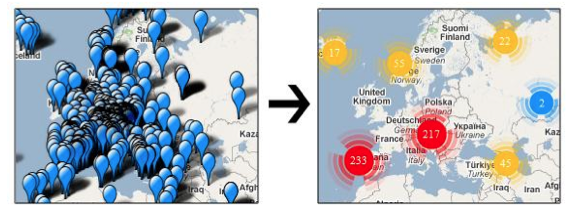
\includegraphics[scale=0.8]{markerclusterer}
	\end{center}
		\legend{Fonte: \cite[figura 20]{silva2010solap+}  }
\end{figure}

		Assim como a biblioteca MarkerClusterer estende a API do Google Maps para uso de agrupamento de marcadores, o plugin Leaflet.MarkerCluster\cite{gitleafletmarker} serve como uma extensão para a API Leaflet. 
		
		Este plugin, faz basicamente as mesmas funções da ferramenta MarkerCluster, porém com algumas melhorias. Por exemplo, ao fazer zoom o mapa exibe uma pequena animação do processo de agrupamento; ao se passar o mouse sobre um marcador do grupo o mapa exibe um polígono que mostra os limites alcançados pelo grupo; os grupos que não são visíveis  na visualização atual do mapa são retirados do mapa para aumentar a performance. Além dessas melhorias, uma que merece destaque é a sua capacidade de customização. 

		Ao contrário da biblioteca MarkerClusterer, o plugin Leaflet.MarkerCluster possui um documentação bastante útil que pode ser encontrada em \cite{gitleafletmarker}. 
		
		É importante observar, que inicialmente, procurou-se por uma documentação mais abrangente da biblioteca MarkerCluster do Google Maps, mas até o momento da confecção desse trabalho não foi possível encontrar nada além de alguns poucos exemplos de uso. Isto, e outros fatores, contribuíram para a escolha da biblioteca Leaflet.js como API de visualização de mapas do framework Searchlight.

\section{Requisitos do Sistema}
Tomando por base o contexto do sistema, foram identificados alguns requisitos para o desenvolvimento do framework Searchlight.


\subsection{Requisitos Funcionais}

\begin{itemize}
\item O framework deve agrupar os marcadores do mapa de forma automática com o objetivo de sumarizar a informação e eliminar a sobreposição de marcadores.

\item O framework deve possuir um mecanismo de zoom que siga a hierarquia de divisão dos agrupamentos. O objetivo desse mecanismo é resolver o problema de zoom arbitrário.

\item O framework deve separar os dados do mapa de acordo com suas categorias por meio de um filtro de categorias. 

\item O framework deve possuir um mecanismo de sumarizar a informação contida num agrupamento. Esse mecanismo deve informar quais categorias estão presentes no grupo e o total de elementos em cada categoria.
\end{itemize}


\subsection{Requisitos Não-Funcionais}
\begin{itemize}
\item Deve-se priorizar a escolha de tecnologias open-source para os componentes externos que forem utilizados pelo framework.
\item O framework deve estar disponível como uma aplicação Web, acessível a partir dos principais navegadores disponíveis no mercado. 
\item O framework deve ser acessível a dispositivos móveis como tablets e smartphones.
\item A interface do framework deve ser de fácil operação, não sendo necessário uso contínuo para uma boa operação.
\end{itemize}

	  

\section{Ferramentas Utilizadas}

Um framework, em desenvolvimento de software, é uma abstração que une códigos comuns entre vários projetos de software provendo uma funcionalidade genérica. Um framework pode atingir uma funcionalidade específica, por configuração, durante a programação de uma aplicação. Ao contrário das bibliotecas, é o framework quem dita o fluxo de controle da aplicação, chamado de Inversão de Controle\footnote{Definição completa em: \url{http://pt.wikipedia.org/wiki/Framework}}.

De modo geral, um framework é conjunto de ferramentas que trabalham em conjunto. O que une as ferramentas são as regras do framework que tem como objetivo prover as funcionalidades que motivaram a criação do dele.

O framework Searchlight tem como objetivo facilitar a criação e a visualização de mapas de crowdsourcing por meio de automatização do processo de criação do mapa. O público alvo abrange  programadores e usuários sem nenhum conhecimento de programação. Para atingir este objetivo o framework faz uso do seguinte conjunto de ferramentas: GitHub, Lealflet.js,  Tabletop.js e RapydScript. 



\subsection{Github\label{github}}
GitHub é um Serviço de Web Hosting Compartilhado para projetos que usam o controle de versionamento Git. Mais do que isso, Github incorpora recursos sociais e de pesquisa que na prática o transformam em uma rede social para programadores. GitHub incorpora elementos tanto do facebook como do twitter. Por exemplo é possível favoritar um projeto, seguir um programador, ver quais sãos as tendências de programação, quais projetos estão se destacando, quais projetos se relacionam entre si e muitos outros recursos.

Neste projeto o github foi usado para hospedar o código fonte da solução desenvolvida e o código latex desta monografia. Todos esses dados podem ser acessados através do endereço \url{https://github.com/wancharle/Searchlight}. 

Na \autoref{fig-gitsource} podemos observar a página do código fonte do projeto. A partir dela um programador pode reportar um bug, solicitar permissões para contribuir com o projeto, copiar o código fonte e muitos outros recursos. 

	\begin{figure}[htb]
	\caption{\label{fig-gitsource}Pagina do github.com que hospeda o código fonte deste projeto.}
	\begin{center}
	    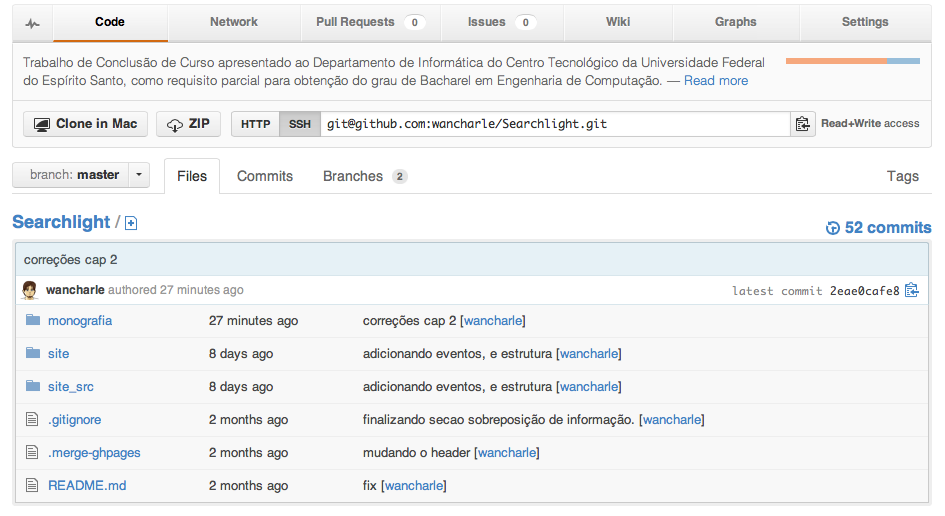
\includegraphics[scale=0.5]{gitsource}
	\end{center}
\end{figure}

Além de hospedar os códigos fontes do projeto, o GitHub também participa ativamente do framework Searchlight. Seu papel no framework é realizado através da ferramenta GitHub Pages. Essa ferramenta estende o uso do GitHub para que ele se comporte como um servidor de páginas web simples. Isto permite ao framework Searchlight hospedar a página de geração e compartilhamento de mapas sem que seja preciso contratar um servidor web apenas para esse propósito.


\subsection{Leaflet.js}

Leaflet é uma biblioteca open-source feita em JavaScript para visualização de mapas interativos. Seu design é baseado em simplicidade, performance e usabilidade. Devido a isso é bastante amigável a dispositivos móveis como tablets e smartphones.

Leaflet é uma biblioteca moderna e robusta, que tira vantagem dos recursos de navegadores modernos como o uso de HTML5  e CSS3 mas ainda mantém suporte aos navegadores antigos.  É bastante confiável e sua estabilidade já foi testada por grandes sites da Web como Foursquare\footnote{Foursquare abandona Google Maps em prol de leaflet.js \url{http://goo.gl/JXPCW}} e Flickr.

Neste projeto, a biblioteca Leaflet é utilizada para fornecer os recursos de exibição e interação com mapas na web.  Além disso, o framework usa a extensão  Leaflet.Spin, para controlar o processo de carregamento de dados, e Leaflet.MarkerCluster, para agrupar marcadores. 

A biblioteca Leaflet foi escolhida considerando os requisitos do sistema e a análise feita em \cite{gmapalternatives} que permitiu a criação da \autoref{tabela-comparativa} que exibe uma comparação entre as sete principais alternativas à  API do Google Maps.

  \begin{table}
  \caption{\label{tabela-comparativa}Comparação entre as principais alternativas à API do Google Maps }
   
  \scalebox{0.8}{   
    \begin{tabular}{|l|l|l|l|}
    \hline
    API            & Dispositivos Móveis  & Renderização         & Diferencial                                                \\ \hline
    Microsoft Bing & Amigável             & Direta               & Perspectiva aérea em vários ângulos           \\
    Nokia          & Amigável             & Direta               & Foco em dispositivos móveis                                \\
    MapQuest       & Amigável             & Direta               & Permite Mapas Licenciados e Mapas Abertos                  \\
    OpenLayers     & Pouco Amigável       & Direta               & Projeto OpenStreetMaps                                     \\
    Leaflet        & Muito Amigável       & Direta ou SVG ou VML & Flexibilidade e Personalização                             \\
    Modest Maps    & Amigável             & Direta               & Design Minimalista.                                        \\
    Polymaps       & Amigável       & SVG                  & Otimizada para grandes volumes de dados. \\ \hline
    \end{tabular}
  }
\end{table}


\subsection{TableTop.js}

Tabletop\cite{tabletop} é uma biblioteca JavaScript que se comunica com o Google Docs e permite a leitura de planilhas eletrônicas por websites via Javascript. 

O framework Searchlight utiliza a biblioteca Tabletop na geração e compartilhamento de mapas. A função da biblioteca, neste caso, é ler as planilhas com as informações do mapa e converter os dados para o formato JSON que é um dos formatos de dados mais utilizado em JavaScript.


\subsection{Rapydscript}

Rapydscript \cite{rapydscript} é um pré-compilador para JavaScript com sintaxe bem próxima da linguagem Python. Sua principal vantagem, é a facilidade de se programar orientado a objetos de forma similar à Python. 

A maior parte do framework Searchlight é escrita usando a sintaxe do Rapydscript. As partes restantes são escritas em JavaScript nativo.

Decidiu-se usar um pré-compilador para JavaScript,  pois a linguagem JavaScript, apesar de ser uma linguagem com suporte a orientação a objetos, não possui uma sintaxe agradável para criação de classes de objetos. Devido a isso, é possível encontrar na internet algumas dezenas de pré-compiladores de javascript\footnote{O site \url{http://altjs.org} exibe uma lista dos principais pré-compiladores de JavaScript.}
. 

\section{Arquitetura do Sistema}
A \autoref{fig-camadas} mostra as camadas que fazem parte da arquitetura do framework Searchlight. A arquitetura do sistema, tal como mostrada na figura, é assim explicada:
	\begin{figure}[htb]
	\caption{\label{fig-camadas}Arquitetura do framework Searchlight.}
	\begin{center}
	    \includegraphics[scale=0.6]{estrutura}
	\end{center}
\end{figure}

\begin{itemize}
\item \textbf{Camada de Aplicação}: é a camada que disponibiliza os serviços do framework aos usuários. Sendo que para usuários programadores a camada disponibiliza a biblioteca Searchlight.js que permite a integração customizada do framework ao website privado do usuário. Porém, para usuários sem conhecimentos de programação, a camada também disponibiliza o gerador de mapas. O gerador de mapas, permite a geração automática de mapas e o seu compartilhamento através da internet sem que seja preciso programar.

\item \textbf{Camada Framework}: é a camada que implementa os serviços oferecidos para os usuários através da camada de aplicação. A camada framework implementa as classes Controle, ClusterCtr e Dados. Essas classes são responsáveis  por controlar a interface de usuário; controlar os agrupamentos, filtros e foco; e pelo processamento de dados do framework. 

\item \textbf{Camada Bibliotecas}: é a camada que implementa  serviços básicos que são utilizados pela camada framework como visualização de mapas, agrupamentos de marcadores e processamento de dados . Os seus principais componentes são a biblioteca Leaflet, com suas extensões, e a biblioteca Tabletop. Sendo que a biblioteca Leaflet é responsável pelas funções visuais do mapa e a biblioteca Tabletop pelo processamento de dados de planilhas do Google Docs.

\item \textbf{Camada Base}: é camada que fornece os componentes estruturais para a construção das camadas superiores. Sendo que os seus principais componentes são o jQuery, para fornecer compatibilidade com  diversos navegadores, e o grupo HTML, CSS e JavaScript que são os blocos estruturais de todo o framework.
 


\end{itemize}

\section{Processamento de dados}
	O processamento de dados do framework Searchlight é feito em duas etapas. Na primeira etapa, o framework faz a leitura dos dados e converte no formato JSON. Na segunda etapa, ele organiza os dados para a utilização nas classes do framework.	
	
	Por convenção, utiliza-se o formato JSON como fonte de dados. A entrada dos dados pode ser feita localmente ou pela internet. Dados que não estejam no formato JSON devem ser processados conforme é mostrado na \autoref{fig-processamento}. 
	
\begin{figure}[htb]
	\caption{\label{fig-processamento}Processamento de dados do framework Searchlight.}
	\begin{center}
	    \includegraphics[scale=0.45]{processamento}
	\end{center}
\end{figure}
	
	Vale ressaltar, que os dados fornecidos localmente são utilizados diretamente pelo framework. Porém,  os dados que são fornecidos via internet precisam ser processados e seguir as regras do protocolo JSONP. 
	
	Arquivos de dados que não estejam no formato JSON podem ser utilizados desde que sejam convertidos e entregues via protocolo JSONP. O framework Searchlight faz essa conversão automaticamente para planilhas do Google Docs. Neste caso, é utilizado a biblioteca Tabletop para converter os dados da planilha para o formato JSON.
	
	Ao passar pela primeira etapa, com os dados já em formato JSON, o framework inicia o processo de organização desses dados. A \autoref{fig-estrutura-de-dados} exibe um diagrama com as estruturas de dados utilizadas e suas classes simplificadas.
		
\begin{figure}[htb]
	\caption{\label{fig-estrutura-de-dados}Estruturas de dados do framework Searchlight.}
	\begin{center}
	    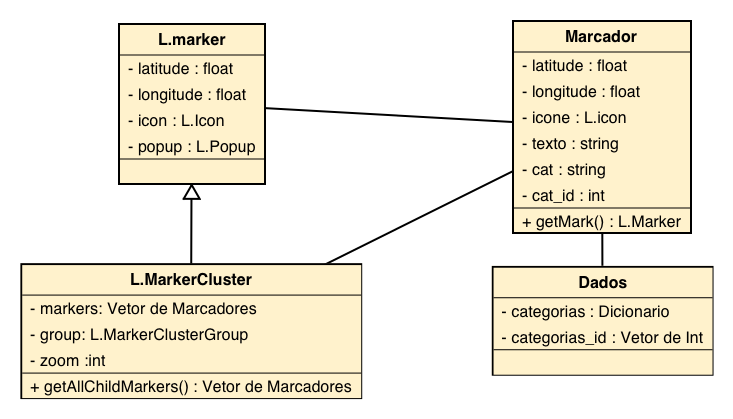
\includegraphics[scale=0.6]{estrutura-de-dados}
	\end{center}
\end{figure}

	De modo geral, a principal estrutura de dados utilizada pelo framework é a arvore de clusters criada pela biblioteca \textit{Leaflet.MarkerCluster}. Esta árvore é representada na \autoref{fig-estrutura-de-dados} pela classe \textit{L.MarkerCluster}. Esta classe herda os dados da classe \textit{L.Marker} que representa marcadores comuns que são exibidos num mapa pela biblioteca \textit{Leaflet}.  
	
	Cada nó dessa arvore é um marcador, cada nível define um novo conjunto de agrupamentos de marcadores, e cada agrupamento está relacionado a um zoom específico. Isso faz com que todos os nós da arvore sejam marcadores virtuais, ou seja, representem apenas agrupamentos de marcadores e não informações concretas. 
	
	As folhas da arvore representam marcadores reais, ou seja, que exibem dados concretos e da fonte dados do mapa. As folhas, são representados na \autoref{fig-estrutura-de-dados} pela classe \textit{Marcador}. Essa classe, é responsável por armazenar informações básicas sobre o marcador e informações extras como categoria do marcador, texto do popup e ícone.  
	
	A classe Dados é responsável por armazenar todos os dados processados na primeira etapa e separá-los em categorias. Para isso utiliza-se um dicionário de categorias. Dessa forma, a chave do dicionário é o nome da categoria, e o valor é uma lista de marcadores que pertencem a essa categoria. Além disso, como recurso para a otimização do framework, também é armazenado uma lista de identificadores numéricos para cada categoria.

	Assim, por meio dessas estruturas de dados é possível controlar o agrupamento de marcadores, popups, zoom  e o filtro de categorias. Além disso, o framework faz uso de outras estruturas de dados que não precisam de pré-processamento. Por exemplo, para desenvolver o recurso de fazer e desfazer ações de zoom é necessário a utilização de algumas variáveis de controle e uma estrutura de pilha para salvar as ações do usuário.  
	
	 
	 
		 
		
